\section{Експеримент}

У овом поглављу описан је експеримент који треба да измери перформансе секвенцијалног, односно паралелног решења.
Такође, представљен је преглед резултата експеримента, то јест, упоредни приказ оба решења.

\subsection{Опис експеримента}

Експеримент описан у овом поглављу треба да измери перформансе секвенцијалног и паралелног решења у различитим случајевима коришћења.

Проблем проналаска суме у бинарном стаблу генерално је веома незахтеван што се тиче процесорских ресурса.
То се дешава због чињенице да је обрада појединачног чвора веома краткотрајна у погледу процесорског времена.
Стога, како би проблем било доследније измерити
\footnote{Приликом иницијалних мерења, оба решења су изузетно брзо долазила до краја извршавања.
Дешавало се да времена извршавања једног решења буду многоструко различита.
То се дешавало због стохастичних процеса попут процесорског кеширања, изборa задатка за извршавање од стране OpenMP библиотеке итд.
који су од извршавања до извршавања били мање или више повољнији.},
у секвенцијално и паралелно решење додато је време обраде појединачног чвора од $1\mu s$.

Паралелно решење покретано је са \textbf{12, 8, 4 и 2 процесуирајуће јединице}.
Бројеви 8, 4 и 2 су изабрани због тога што су то степени броја два тј. бројеви чворова на нивоима 3, 2 и 1 бинарног стабла, респективно, те ова решења нуде
могућност паралелне обраде $l$ чворова. Међутим, решење је покретано и са 12 ПЈ, јер се при иницијалним мерењима показала предност покретања паралелног решења
и са бројем ПЈ који није умножак двојке, а која се своди на следеће: сви OpenMP задаци у паралелном решењу познати су тек када сви задаци на нивоу $l-1$ започну
своје извршавање и генеришу те задатке; OpenMP извршно окружење стохастично извршава задатке те је чест случај да чвор на нивоу $l-1$ ни не крене да се извршава
док неки од чворова нивоа $l$ не заврше своју обраду. Стога, што више ПЈ, то је већа вероватноћа да ће распоређивач извршити чвор нивоа $l-1$ и креирати задатке.

Решења су покретана над стаблима величина 10 чворова (пример са слике \ref{fig:primersume}), 10 хиљада чворова и 100 хиљада чворова.
Тражена сума је бирана тако да:
\begin{enumerate}
    \item Решење не постоји.
    \item Сума се налази на путањи састављеној од све леве деце-чворова (оптималан случај секвенцијалног решења). Означено као \textbf{решење Л}.
    \item Сума се налази на путањи састављеној од деце-чворова биране тако да се наизменично бирају лево и десно дете-чвор (погодан случај паралелног решења са већим бројем ПЈ).
    Означено је као \textbf{решење С}.
\end{enumerate}

\subsection{Резултати}

На сликама \ref{fig:rez10}, \ref{fig:rez10k} и \ref{fig:rez100k} приказане су брзине извршавања решења у односу на растући број процесуирајућих јединица.
Секвенцијално решење представљено је подацима о извршавању са 1 процесуирајућом јединицом.

\begin{figure}[]
    \centering
    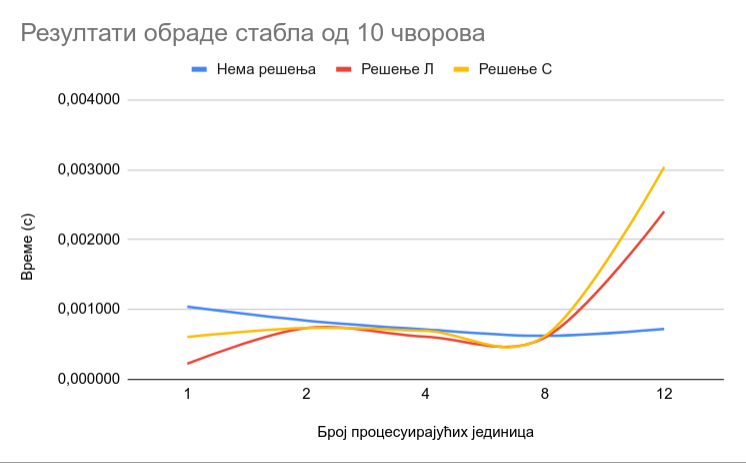
\includegraphics[scale = 0.7]{rezultat-10-cvorova.png}
    \caption{Резултати обраде стабла величине 10 чворова}
    \label{fig:rez10}
\end{figure}

\textbf{Паралелно решење у општем случају није брже обрадило стабло величине 10 чворова}.
Штавише, обрада стабла од 10 чворова употребом 12 процесуирајућих јединица довело је до знатно лошијих перформанси.
Ово се може објаснити тиме да је додатно време које паралелно решење троши на креирање OpenMP задатака, а које потом и то извршно окружење троши за
управљање животним циклусом задатка исувише велико у односу на количину рада потребну за обраду тако малог стабла.

Исто објашњење важи и за резултате са 2, 4 и 8 ПЈ, с тим што је за случај у коме нема решења, већ евидентна предност паралелног
над секвенцијалним решењем. Овај случај подразумева да се обиђу сви чворови у графу и, стога, повољнији је за паралелну обраду.

Решење Л очекивано фаворизује секвенцијалну обраду.

\begin{figure}[]
    \centering
    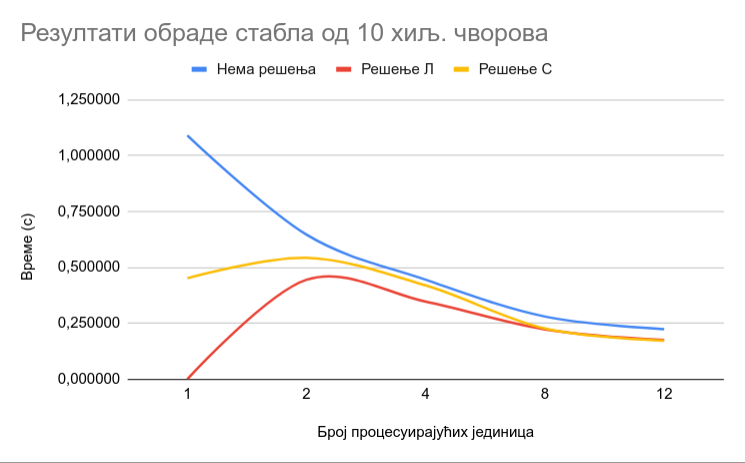
\includegraphics[scale = 0.7]{rezultat-10k-cvorova.png}
    \caption{Резултати обраде стабла величине 10 хиљада чворова}
    \label{fig:rez10k}
\end{figure}

\begin{figure}[]
    \centering
    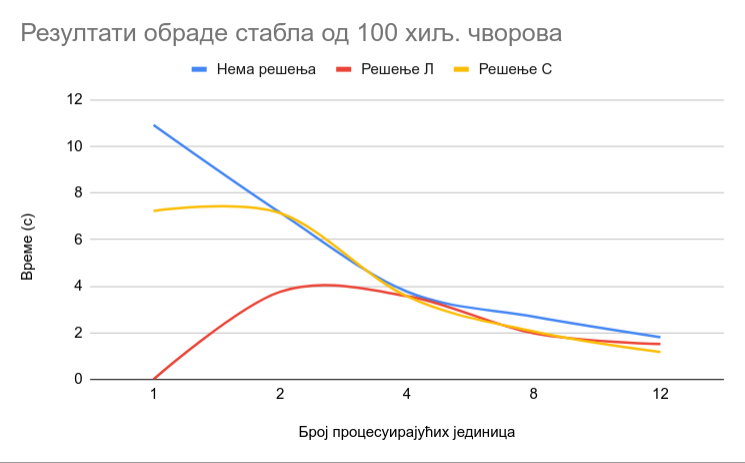
\includegraphics[scale = 0.7]{rezultat-100k-cvorova.png}
    \caption{Резултати обраде стабла величине 100 хиљада чворова}
    \label{fig:rez100k}
\end{figure}

Резултати обрада стабала од 10 и 100 хиљада чворова су веома слични.

\textbf{Евидентно је да се са порастом броја процесуирајућих јединица брже долази до решења у општем случају}.
Ово без изузетка важи за случај у коме нема решења.

Паралелно решење за случај решења С са 2 ПЈ не нуди веће убрзање од секвенцијалног решења.
Ово се може објаснити тиме што секвенцијално решење обиђе пола стабла како би дошло до решења С,
док паралелно решење обиђе читаво стабло, али се обрада појединачне половине стабла извршава секвенцијално, у засебној ПЈ.
Стога, брзине проналаска решења С су једнаке.


\pagebreak